\documentclass[
    linespread = 1.25
]{ctexart}
\pagestyle{plain}
\ctexset{
    section/format = \Large\bfseries\raggedright,
    section/number = {\chinese{section}、},
    section/aftername = {\enskip},
    abstractname = {\zihao{-2}摘\quad 要}
}
\usepackage[table,xcdraw]{xcolor}
\usepackage[a4paper, lmargin=1in, rmargin=1in, tmargin=1in, bmargin=1in]{geometry}
\usepackage{amsmath}
\usepackage{booktabs}
\usepackage{graphicx}
\graphicspath{ {./fig} }

\usepackage{listings}
\usepackage{color}

\usepackage[sorting=none]{biblatex}
\addbibresource{LLMTuningReport.bib}

\definecolor{dkgreen}{rgb}{0,0.6,0}
\definecolor{gray}{rgb}{0.5,0.5,0.5}
\definecolor{mauve}{rgb}{0.58,0,0.82}

\lstset{
  frame=tb,
  language=Python,
  aboveskip=3mm,
  belowskip=3mm,
  showstringspaces=false,
  columns=flexible,
  basicstyle={\small\ttfamily},
  numbers=left,
  numberstyle=\tiny\color{gray},
  keywordstyle=\color{blue},
  commentstyle=\color{dkgreen},
  stringstyle=\color{mauve},
  breaklines=true,
  breakatwhitespace=true,
  tabsize=2
}
\usepackage{amssymb}
\usepackage[hidelinks]{hyperref}
\usepackage{caption}
\usepackage{subcaption}
\usepackage{siunitx}
\usepackage{algorithm2e}
\SetAlgoInsideSkip{bigskip}
\SetAlgorithmName{算法}{算法}{算法}
\RestyleAlgo{ruled}
\usepackage{multicol}
\usepackage{longtable}
\usepackage{tablefootnote}
\usepackage{float}


\title{\zihao{2}\textbf{大数据创新实践实验报告}\\\zihao{3}\textbf{——多模态大模型LLaVA的微调}}
\author{\zihao{4}曹瀚文 \\\texttt{学号:210810503}
\and \zihao{4}岑畅 \\\texttt{学号:210810501}
\and \zihao{4}丁有罡 \\\texttt{学号:210810518}
\and \zihao{4}符永宣\\\texttt{学号:210810506}
\and \zihao{4}金文韬\\\texttt{学号:210810306}
\and \zihao{4}刘炎培\\\texttt{学号:210810510}
\and \zihao{4}刘梓涛\\\texttt{学号:210810513}
\and \zihao{4}彭珂\\\texttt{学号:210810508}
\and \zihao{4}王子霖\\\texttt{学号:210810522}
\and \zihao{4}文宇祥\\\texttt{学号:210810514}
}
\date{}

\begin{document}

\begin{titlepage}
  \newgeometry{top=1in,bottom=1in,right=0.75in,left=0.75in}
  \maketitle
  \vspace{0.2cm}
  \begin{abstract}
    \zihao{-4}
    \vspace{0.8cm}
    \linespread{1.25}
    本论文主要研究了空气质量、污染物水平及其与时空、气候因素的关系,并基于历史数据预测未来空气质量。论文首先对数据进行了预处理,包括数据描述、数据标准化、异常值及缺失值处理、极值值处理等步骤。接着,采用系统聚类方法对不同城市的污染物水平进行了潜在模式探索,通过均值和不同邻距离的聚类方法分析得出了系统聚类结果,并用因子分析的得分对其进行了解释。

    论文进一步探讨了空气质量与时空、气候因素的相关关系,应用多元线性回归模型和改进的多元线性回归模型,诊断模型结果并分析了气候因素与空气质量之间的相关性。此外,论文介绍并应用了广义线性模型,实现利用时空、气候因素对空气质量进行更加准确的预测。

    最后,论文利用SARIMA模型和GARCH模型,根据历史空气质量数据预测未来一段时间内的空气质量,以南昌市为例进行了实证研究。通过数据导入、探索性期性、参数确定、模型诊断及预测等步骤,详细展示了两种模型的应用过程和预测效果。

    本文不仅揭示了不同城市空气污染物可能存在的潜在模式,同时探究了空气质量与多种因素之间的复杂关系,也为空气质量的预测提供了有效的模型和方法,对城市环境管理、污染控制和空气质量的预报具有重要的参考价值。

    \vspace{1cm}
    \noindent\textbf{关键词:} 系统聚类\hspace{0.22cm} 因子分析\hspace{0.22cm} 多元线性回归\hspace{0.22cm} 广义线性模型\hspace{0.22cm} 时间序列分析
  \end{abstract}
\end{titlepage}

\tableofcontents
\newpage
\section{实验背景}
在当今人工智能和机器学习领域,预训练大规模语言模型(如GPT-4)已经展现出卓越的性能。然而,尽管这些模型在许多任务中表现优异,它们的通用性仍然可能无法满足特定应用场景的需求。因此,为了进一步提升模型在特定领域的效果,参数微调成为了一个关键的研究方向。通过微调,我们可以根据特定的数据集和任务需求对模型进行定制,使其在处理特定类型的输入时表现得更加精准和高效。这种方法不仅可以改善模型的预测能力,还能提升其对领域特定知识的理解和应用能力。为了实现最佳的微调效果,研究者们通常需要细致地调整模型的超参数,探索不同的优化策略,以便找到最适合特定应用场景的配置。

本次参数微调实验旨在通过自动驾驶数据集对LLaVA模型进行微调,以期提升该模型在自动驾驶领域的综合表现。同时,在该过程中我们希望探究微调过程中的关键影响因素,并采用多种方法评估微调效果。

本次实验选取的模型是开源的大语言模型LLaVA\cite{liu2023llava},该模型结合了语言模型和视觉模型,能够同时处理文本和图像输入,从而更好地理解和生成多模态信息,如图\ref{fig:LLaVA}所示。LLaVA通过大规模预训练学习到丰富的特征表示,并在特定任务中通过微调进一步优化性能,在自动驾驶、医疗影像分析、智能客服和内容创作等多个领域展现出广泛的应用前景和高效的推理性能。

本次实验将采用的是LoRA(Low-Rank Adaptation)参数微调算法\cite{hu2021loralowrankadaptationlarge},它是一种高效的参数微调方法,通过在预训练模型的权重矩阵上添加低秩分解来减少参数数量,如图\ref{fig:LoRA}所示。这种方法不仅显著降低了微调过程中所需的计算资源和存储空间,还能在保持模型性能的同时,快速适应新的任务和数据。LoRA通过只微调一小部分参数,使得大规模预训练模型的应用更加灵活和经济。

\begin{figure}[htbp]
  \centering
  \begin{minipage}[b]{0.6\textwidth}
    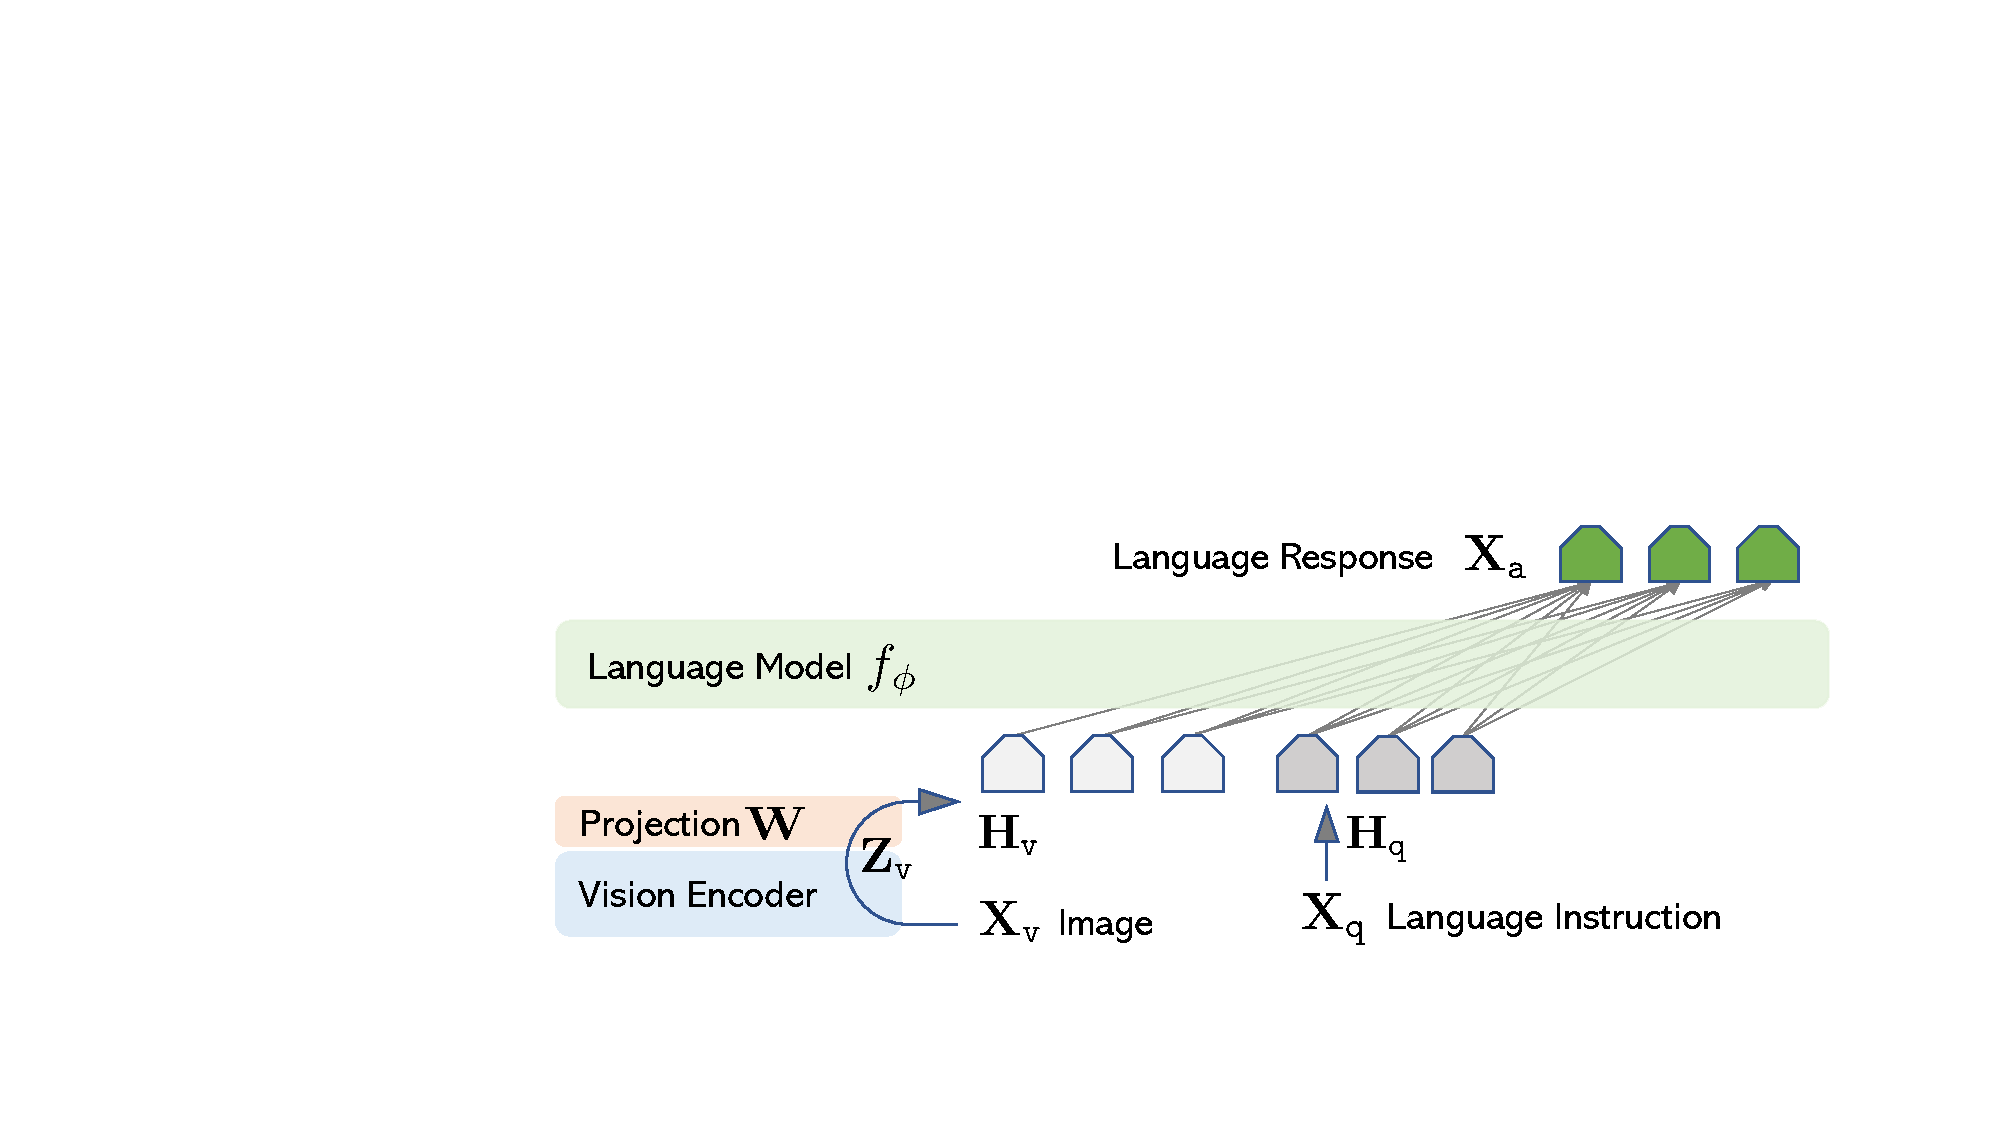
\includegraphics[width=\textwidth]{illu_llava.pdf}
    \caption{LLaVA模型架构}
    \label{fig:LLaVA}
  \end{minipage}
  \hfill
  \begin{minipage}[b]{0.25\textwidth}
    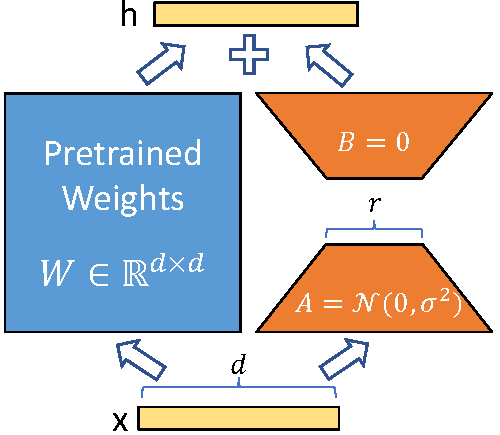
\includegraphics[width=\textwidth]{illu_lora.pdf}
    \caption{LoRA算法图解}
    \label{fig:LoRA}
  \end{minipage}
\end{figure}

% 本次实验在黎勃老师提供的Linux服务器平台上进行,通过SSH远程连接服务器进行实验。

\section{基于自动驾驶数据集的模型微调}

% \subsection{LoRA参数微调算法简介}
% 这段全是GPT写的, 哪个哥们看着改一下吧

% LoRA(Low-Rank Adaptation of Large Language Models)是一种用于微调大型语言模型的算法,旨在减少微调过程中的计算和存储开销。LoRA通过引入低秩矩阵来调整模型的权重,而不是对整个模型进行完全微调。这种方法特别适用于需要在有限资源下进行高效微调的场景。

% \subsubsection{LoRA算法的核心概念}

% \begin{enumerate}
%   \item \textbf{低秩矩阵分解}:
%     \begin{itemize}
%       \item LoRA利用低秩矩阵分解(Low-Rank Decomposition)来表示权重矩阵的变化。具体来说,给定一个权重矩阵$W$,LoRA将其表示为两个低秩矩阵$A$和$B$的乘积,即$W + \Delta W \approx W + A \cdot B$,其中$\Delta W$是权重的调整部分。
%     \end{itemize}
%   \item \textbf{参数高效性}:
%     \begin{itemize}
%       \item 通过使用低秩矩阵,LoRA显著减少了需要学习的参数数量。这不仅降低了存储需求,还减少了训练和推理的计算开销。
%     \end{itemize}
%   \item \textbf{保持原模型的冻结状态}:
%     \begin{itemize}
%       \item 在LoRA中,原始模型的权重保持冻结状态,只有低秩矩阵$A$和$B$会在微调过程中进行更新。这使得LoRA在微调过程中能够更好地保持原始模型的特性,同时适应新的任务需求。
%     \end{itemize}
% \end{enumerate}

% \subsubsection{LoRA的工作流程}

% \begin{enumerate}
%   \item \textbf{初始化低秩矩阵}:
%     \begin{itemize}
%       \item 在开始微调之前,LoRA初始化两个低秩矩阵$A$和$B$,它们的维度通常远小于原始权重矩阵$W$。
%     \end{itemize}
%   \item \textbf{微调过程}:
%     \begin{itemize}
%       \item 在微调过程中,仅对低秩矩阵$A$和$B$进行更新,原始权重矩阵$W$保持不变。通过梯度下降法,优化目标函数以最小化模型在新任务上的损失。
%     \end{itemize}
%   \item \textbf{预测和推理}:
%     \begin{itemize}
%       \item 在推理阶段,将更新后的低秩矩阵与原始权重矩阵结合,生成最终的权重$W' = W + A \cdot B$,用于模型预测。
%     \end{itemize}
% \end{enumerate}

% \subsubsection{LoRA的优点}

% \begin{enumerate}
%   \item \textbf{参数效率}:
%     \begin{itemize}
%       \item LoRA通过引入低秩矩阵显著减少了需要更新的参数数量,使得微调过程更为高效。
%     \end{itemize}
%   \item \textbf{资源节省}:
%     \begin{itemize}
%       \item 由于只需更新较小的低秩矩阵,LoRA在存储和计算资源上的需求较低,非常适合在资源受限的环境中进行微调。
%     \end{itemize}
%   \item \textbf{保持原始模型特性}:
%     \begin{itemize}
%       \item LoRA在微调过程中冻结了原始模型的权重,这有助于保持原始模型的特性和性能。
%     \end{itemize}
% \end{enumerate}

% \subsubsection{LoRA在实践中的应用}

% LoRA已经在多个自然语言处理(NLP)任务中得到了应用,例如文本分类、情感分析和机器翻译。它特别适用于大规模预训练模型的微调,例如BERT、GPT和T5等。

% 通过使用LoRA,开发者可以在保持模型高性能的同时,大幅减少微调所需的计算和存储资源,使得大模型的应用更加广泛和便捷。

\subsection{使用LoRA算法和自动驾驶数据集对LLaVA模型作指令微调}
我们对llava-v1.5-7b和llava-v1.5-13b两个模型使用了LoRA算法进行微调,两个模型的区别在于规模大小,其中7b模型的参数量为70亿,13b模型的参数量为130亿。

我们使用的数据集是\texttt{bdd1k\_by\_Qiancai}。该数据集由王前才学长提供,衍生自开源的自动驾驶图片数据集\texttt{BDD100k}\cite{yu2020bdd100kdiversedrivingdataset},从中选取的1000张图片尽可能地覆盖了各种驾驶场景,
并借助商业多模态模型辅助了生成图像-文本对数据集,经人工检查保证了数据集质量。

我们使用的微调方法是LLaVA官方提供的微调脚本。为使微调效果更佳,我们通过尝试修改了一些训练参数。对上述两个模型分别进行了10个epoch的微调,微调过程中的损失函数变化如图\ref{fig:7b规模模型训练过程中的loss}、\ref{fig:13b规模模型训练过程中的loss}所示。可以看到,随着模型微调轮数的增加,模型的损失函数逐渐下降,表明模型在训练过程中逐渐收敛。
\begin{figure}[H]
  \centering
  \begin{subfigure}{0.49\textwidth}
    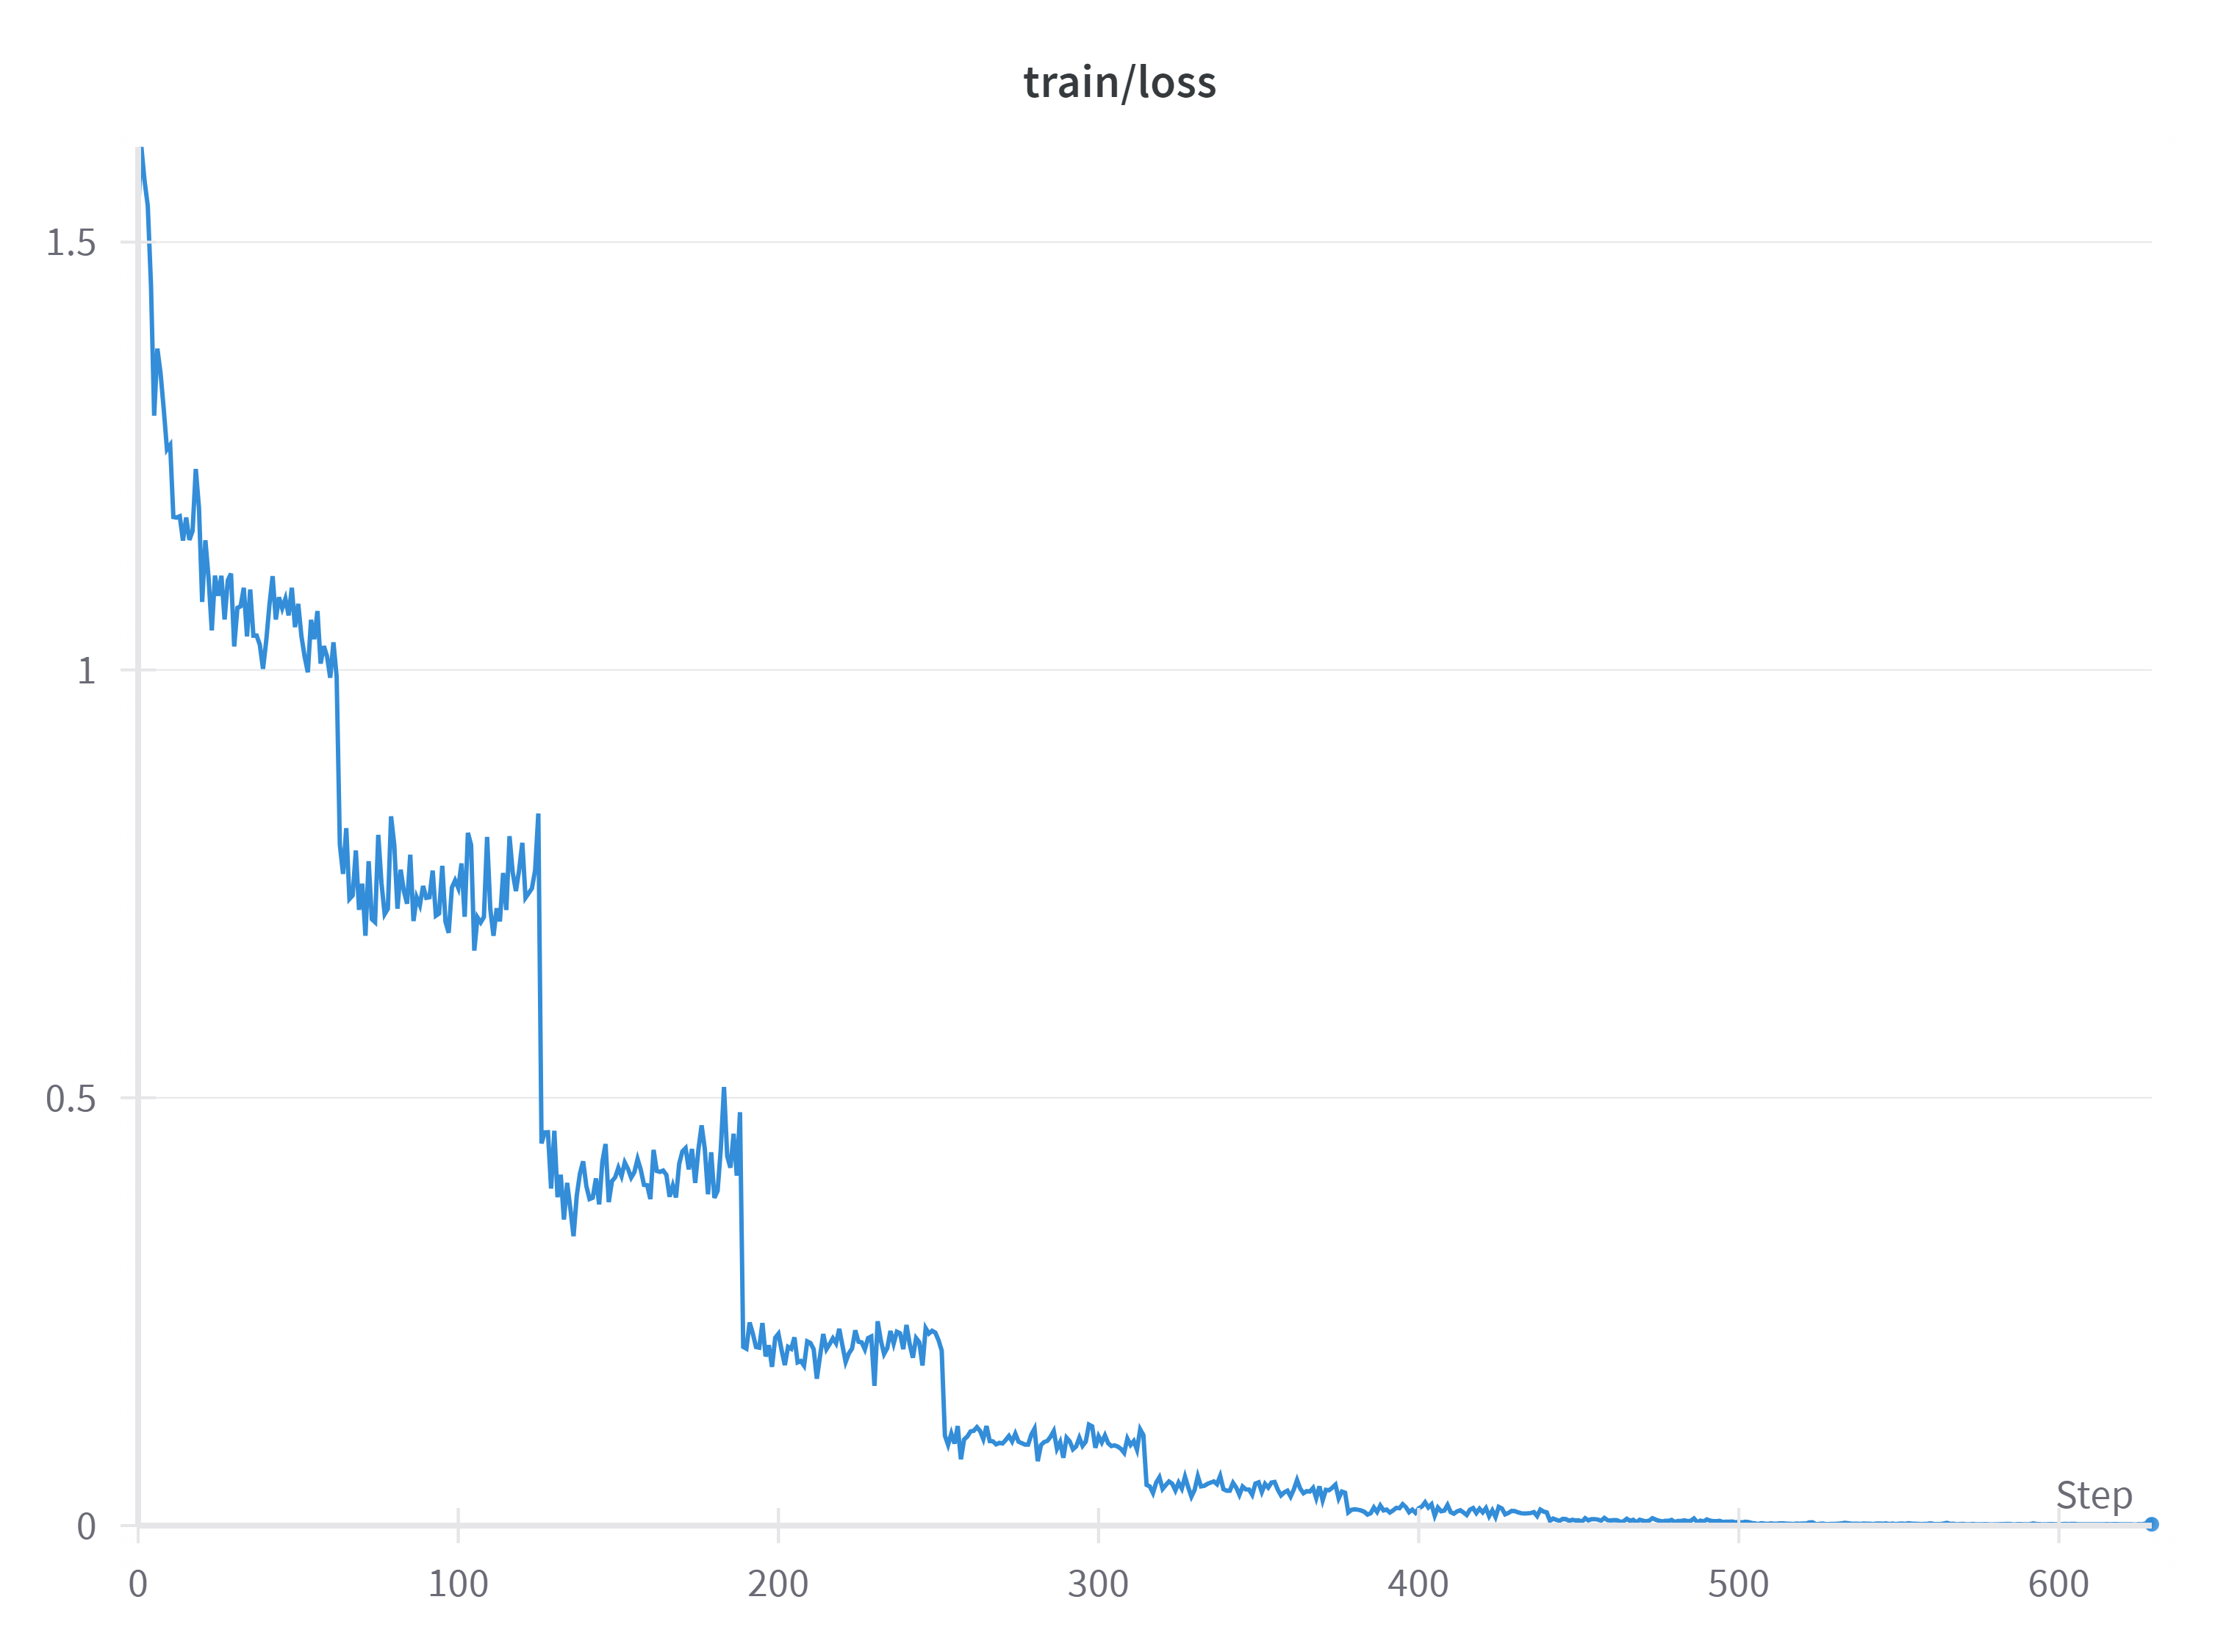
\includegraphics[width=\textwidth]{7b.png}
    \caption{7b规模模型}
    \label{fig:7b规模模型训练过程中的loss}
  \end{subfigure}
  \hfill
  \begin{subfigure}{0.49\textwidth}
    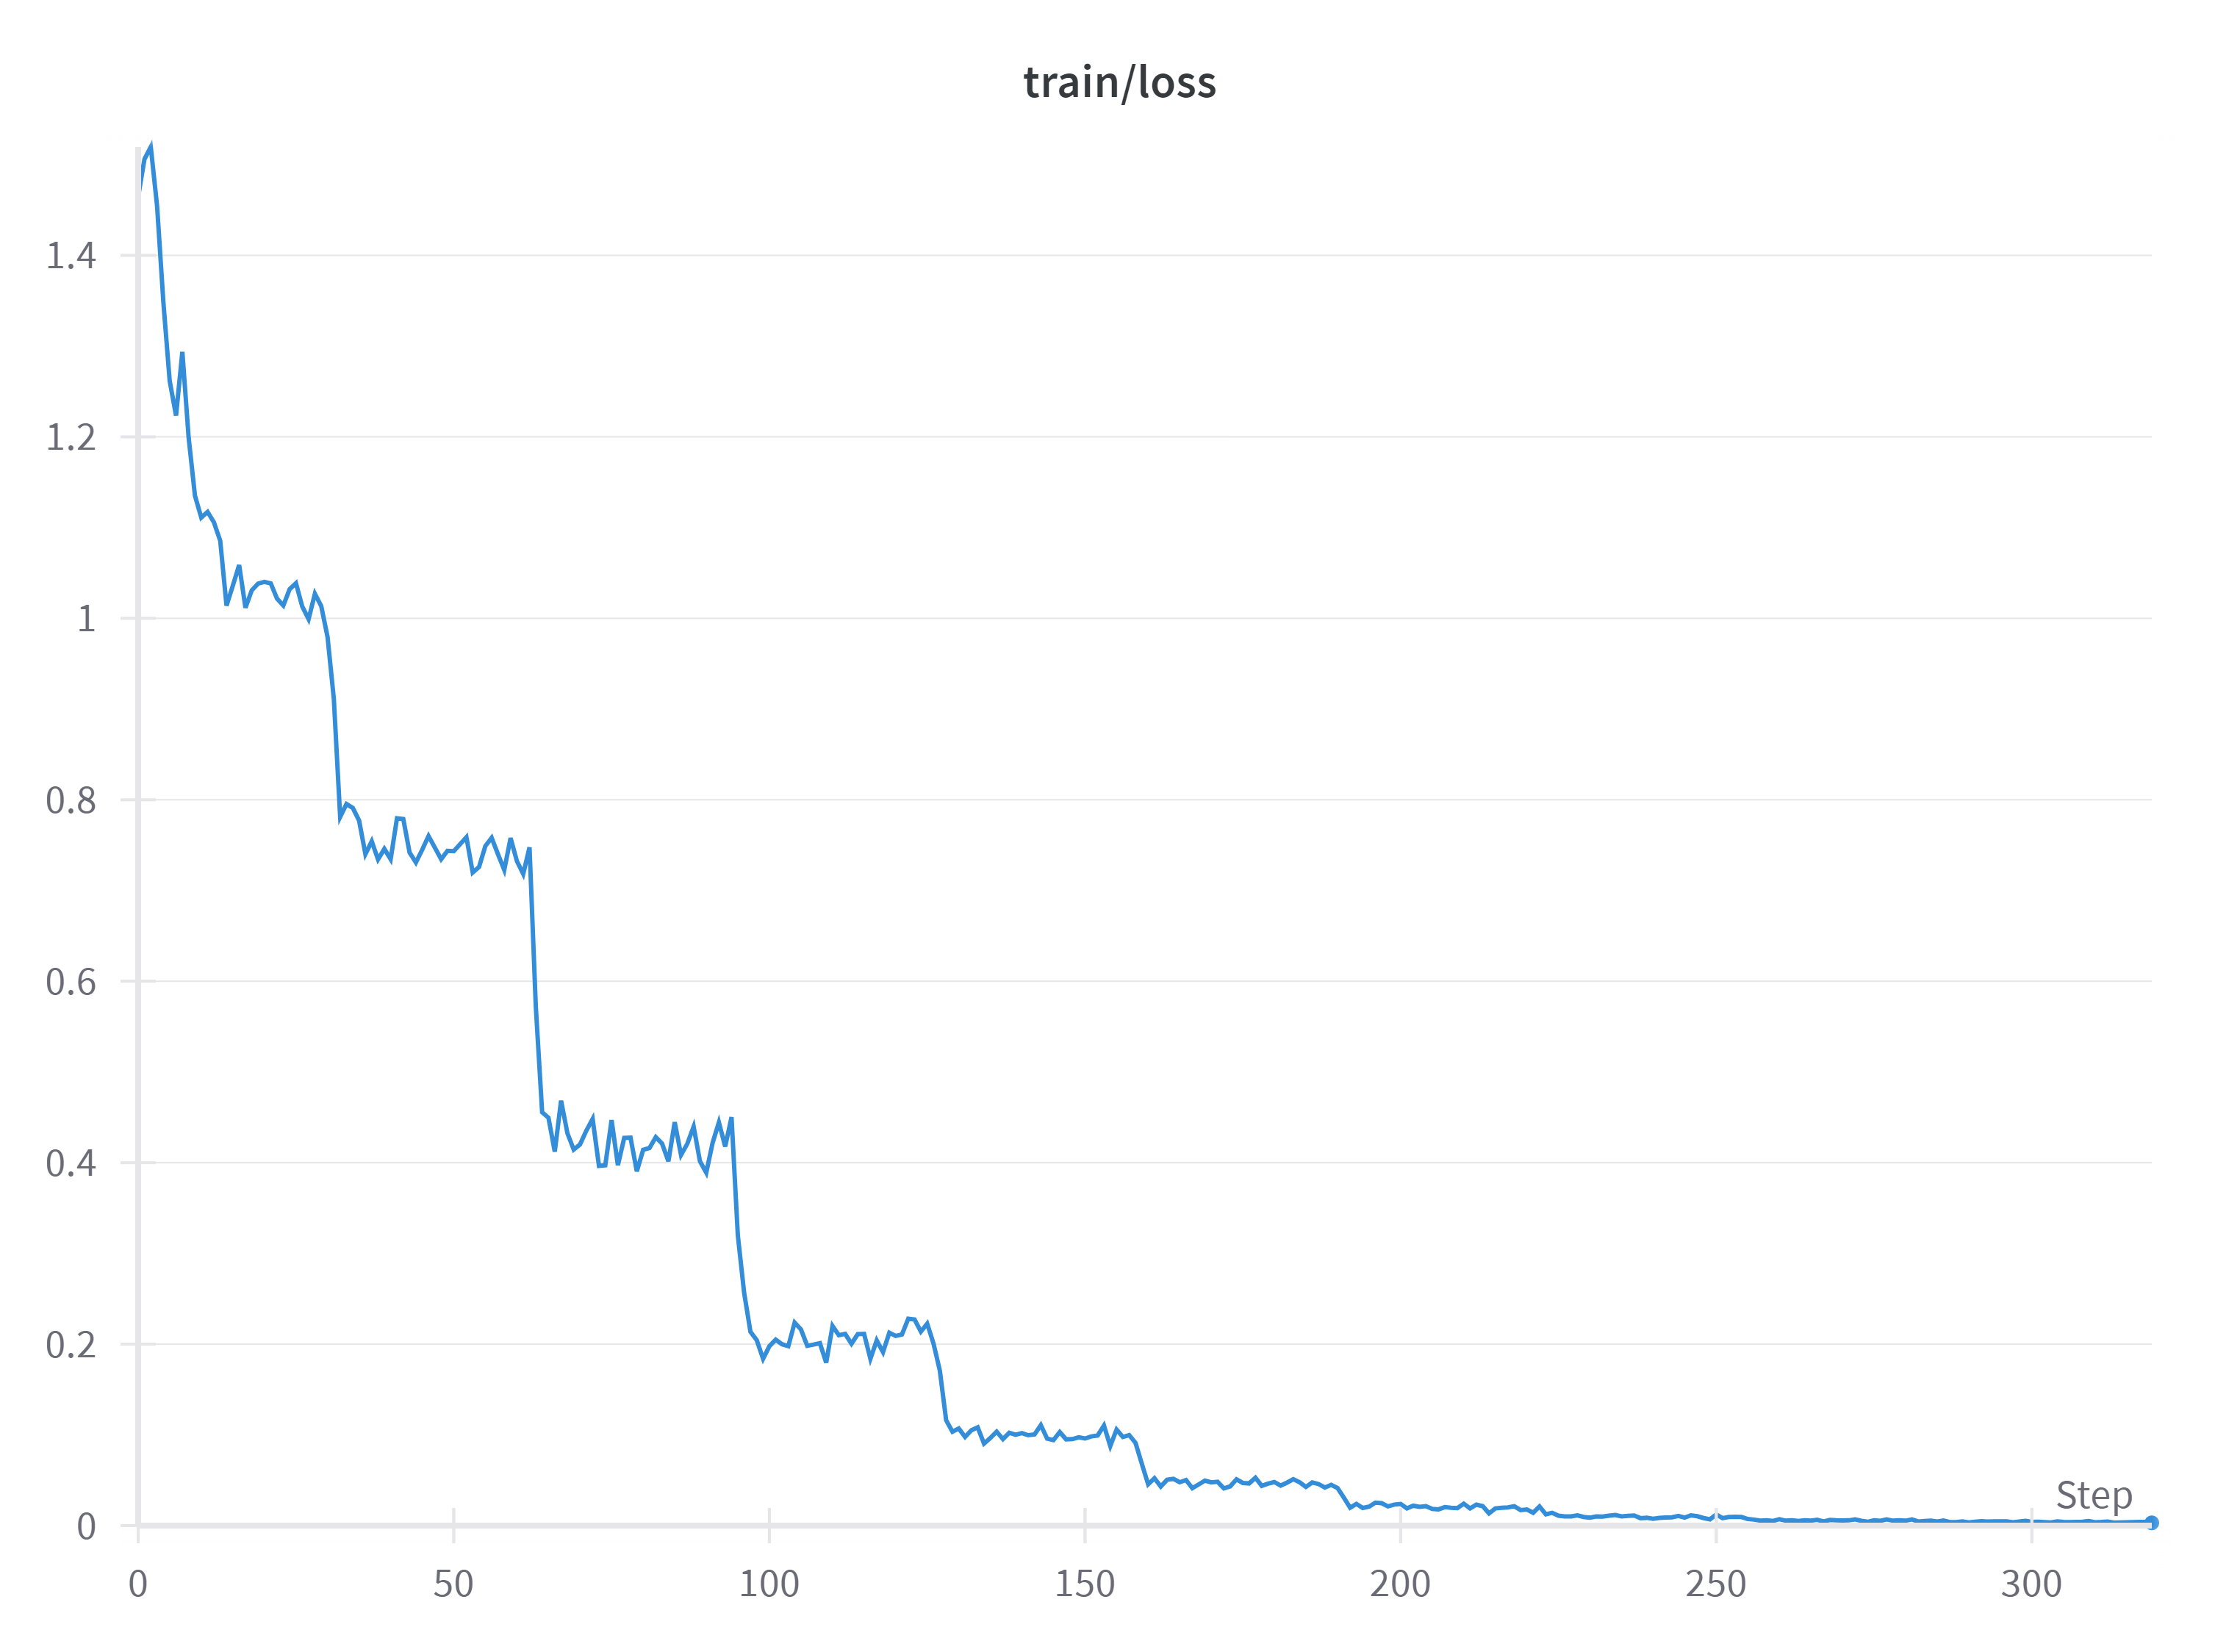
\includegraphics[width=\textwidth]{13b.png}
    \caption{13b规模模型}
    \label{fig:13b规模模型训练过程中的loss}
  \end{subfigure}
  \caption{模型训练过程中的损失函数变化}
  \label{fig:模型训练过程中的loss}
\end{figure}


\subsection{实现微调模型的图形化界面}
开源的LLaVA模型提供的交互接口较为原始,每一步调用都需要通过命令行传递模型的路径、训练结果的路径等相关参数,且难以实现连续的对话。

为了方便模型的后续调用与测试,我们对参数微调后的LLaVA模型进行了适当封装,并借助Python的curses库制作了一个朴素的GUI界面进行模型的调用,如图\ref{fig:gui_result}所示。用户可以通过该界面选择使用的模型微调版本、输入图片路径,并与模型进行连续对话,如图\ref{fig:result}所示。

通过GUI界面图\ref{fig:gui}可以清楚地看到,模型在我们给出的示例图片上的回答可以令人满意。
\begin{figure}[htbp]
  \centering
  \begin{subfigure}{0.6\textwidth}
    \centering
    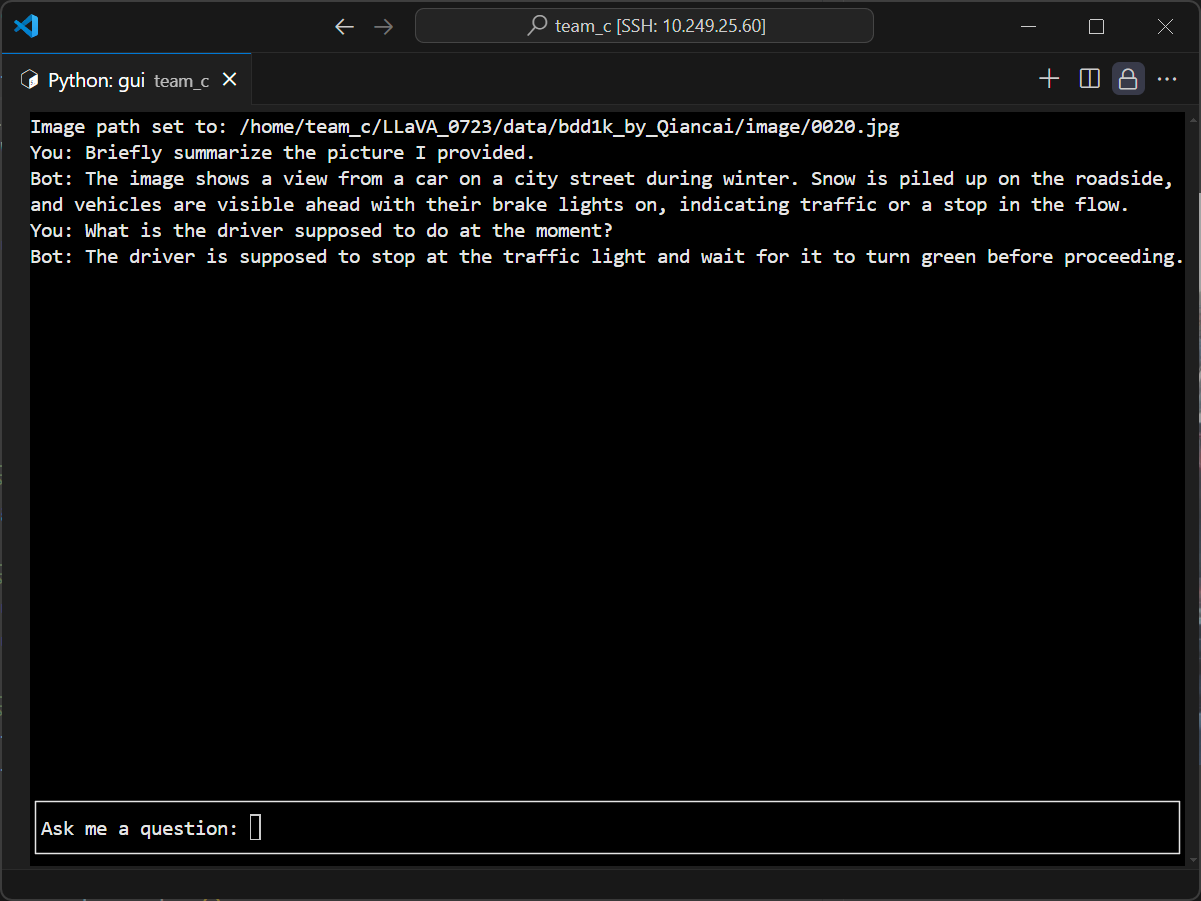
\includegraphics[width=\textwidth]{gui.png}
    \caption{GUI界面}
    \label{fig:gui}
  \end{subfigure}
  \hfill
  \begin{subfigure}{0.36\textwidth}
    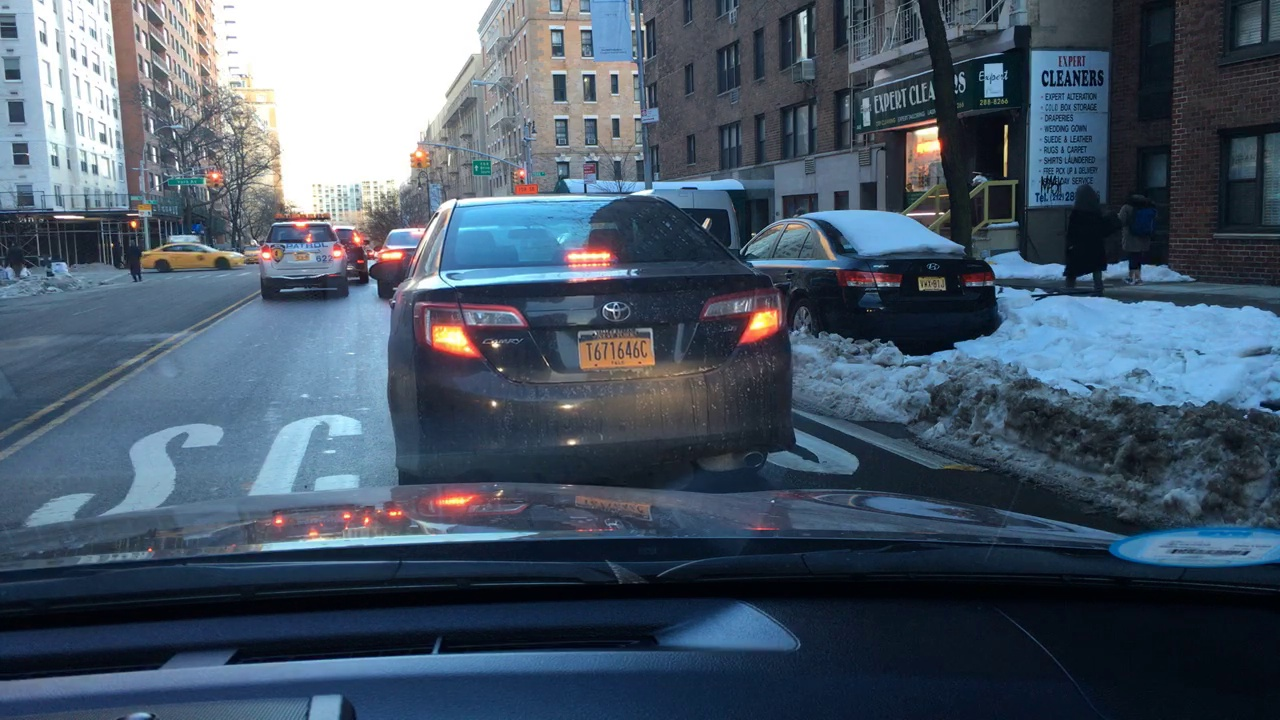
\includegraphics[width=\textwidth]{0020.jpg}
    \caption{示例图片\texttt{0020.jpg}}
    \label{fig:result}
  \end{subfigure}
  \caption{GUI界面运行示例}
  \label{fig:gui_result}
\end{figure}

\subsection{结论}

本次实验中,我们使用LoRA算法,利用自动驾驶数据集对LLaVA模型进行了指令微调。我们对两个不同规模的LLaVA模型进行了微调,分别是7b规模和13b规模的模型。通过微调过程中的损失函数变化,我们可以看到模型在训练过程中逐渐收敛,表明模型的微调效果较好。

此外,我们还实现了一个简单的GUI界面,方便用户调用不同微调后的LLaVA模型进行连续对话。通过该界面,用户可以选择使用的模型版本、输入图片路径,并与模型进行连续对话,实现了模型的可视化调用。

\section{初步评估微调结果并探究影响微调效果的试验因素}
\subsection{使用VizWiz数据集评估微调模型的通用性能}

\subsubsection{数据集介绍}

VizWiz是一个用于视觉问题回答(VQA)任务的大型数据集\cite{gurari2018vizwizgrandchallengeanswering},旨在帮助盲人和视障人士获取有关他们周围环境的信息,被广泛应用于多模态大模型通用性能的评估。该数据集包含了来自视障用户的手机拍摄的图片,用户通过语音提问的方式获取图片中的信息。VizWiz数据集中的问题通常涉及图片中的物体、场景、颜色等内容,需要模型结合图片信息和问题描述给出准确的回答。

我们将微调后的不同模型应用于VizWiz数据集,通过评估模型在VQA任务上的表现,探究微调效果的影响因素。我们选取的模型包括两种参数规模:7b和13b,以及三种训练周期:0 epoch(baseline)、5 epochs和10 epochs。通过对比不同模型和微调方法的表现,我们可以更好地理解指令微调对模型通用性能的影响,为模型选择和微调提供参考。

\subsubsection{评估结果}

不同模型在VizWiz数据集上的测试得分如表\ref{tab:vizwiz}所示。关于表\ref{tab:vizwiz},以下观察值得注意:
\begin{itemize}
  \item 不论是7b规模还是13b规模的模型,微调后的模型在VizWiz数据集上的表现均不如未微调的baseline模型。这可能是由于我们的微调指令为自动驾驶方面的数据集,虽然能够提高模型在自动驾驶领域的表现,但对于其他领域的通用性能可能带来负面效果。
  \item 不论是7b规模还是13b规模的模型,10个epoch的训练周期相比于5个epoch的训练周期,微调效果都出现了一定程度的下降。这可能是由于训练周期过长导致模型过拟合,从而影响了模型在VQA任务上的表现。
  \item 相比7b规模的模型,13b规模的模型在VizWiz数据集上的表现整体更好。这可能是由于13b规模的模型具有更多的参数和更强的表达能力,能够更好地理解和生成多模态信息,从而在VQA任务上表现更佳。
\end{itemize}

\begin{table}[hbt]
  \centering
  \caption{VizWiz数据集的测试得分}
  \label{tab:vizwiz}
  \begin{tabular}{@{}llllll@{}}
  \toprule
  Model            & Overall & Yes/No & Number & Unanswerable & Other \\ \midrule
  \texttt{7b-0epoch}   & 50.38   & 78.34  & 46.02  & 75.39        & 38.69 \\
  \texttt{7b-5epoch}   & 48.77   & 68.17  & 29.43  & 94.65        & 29.65 \\
  \texttt{7b-10epoch}  & 48.32   & 65.42  & 28.62  & 93.99        & 29.43 \\
  \texttt{13b-0epoch}  & 54.32   & 79.28  & 42.76  & 68.23        & 47.42 \\
  \texttt{13b-5epoch}  & 47.99   & 75.33  & 41.14  & 56.09        & 43.14 \\
  \texttt{13b-10epoch} & 47.78   & 75.3   & 41.71  & 57.83        & 42.13 \\ \bottomrule
  \end{tabular}
\end{table}

\subsection{影响微调效果的实验因素}

\subsubsection{探究训练周期对微调效果的影响}

\subsubsection{探究模型大小对微调效果的影响}

\subsection{结论}

\section{使用CODA-LM数据集评估微调模型在自动驾驶领域的性能}
\subsection{数据集介绍}
CODA-LM 是一个用于自动驾驶边缘情况的大型视觉语言模型(Large Vision-Language Models)评估基准。这个数据集采用分层数据结构,可以促使LVLMs分析复杂的驾驶场景,并生成高质量的预注释供人工注释者进一步验证和修订。CODA-LM旨在提供一个自动化和量化的评估方法,用于解决自动驾驶系统在处理真实世界的边缘情况时常见的挑战。

如表\ref{CODA-LM dataset}中所示,CODA-LM 是首个采用分层评估框架的大规模多模式自动驾驶道路拐角案例数据集 \cite{chen2024automatedevaluationlargevisionlanguage}。其中包含了三种任务:一般感知、区域感知和驾驶建议。为了更好地理解CODA-LM数据集的评估指标,我们详细介绍一下这三个任务:

\begin{enumerate}
  \item \textbf{一般感知 (General Perception):}
        这个任务的基础在于全面理解驾驶场景中关键的道路实体,包括它们的外观、位置,以及它们如何影响自我车辆的驾驶行为。这个任务对于评估大型视觉语言模型(LVLMs)在解释复杂交互场景中的熟练程度至关重要,仿佛在镜像自动驾驶中的感知过程。此外,为了全面评估LVLMs在不同环境下的表现,数据集根据时间和天气条件对图像进行分类,包括夜间和白天场景,以及晴朗、多云和雨天的天气条件。

  \item \textbf{区域感知 (Regional Perception):}
        这个任务衡量LVLMs在提供特定边界框时理解边缘案例对象的能力,涉及描述给定边界框内的对象以及解释它们为何会影响自动驾驶行为。建立区域感知基于一个核心认识——精确定位边缘案例对于提高系统在自动驾驶实际应用中的整体稳健性至关重要。这些情景通常包含复杂或不寻常的元素,传统模型可能会忽视或难以正确解释,例如独特的交通标志、行为异常的行人和非典型的道路条件。通过专注于这些案例,可以全面了解模型理解边缘案例对象的能力。

  \item \textbf{驾驶建议 (Driving Suggestions):}
        这个任务旨在评估LVLMs制定驾驶建议的能力,这是可解释自动驾驶的一个关键组成部分。这个任务与自动驾驶的规划过程密切相关,要求模型在正确感知当前驾驶环境的一般和区域方面后,为自我车辆提供最佳的驾驶建议。通过构建驾驶建议任务,可以深入评估LVLMs在制定有效驾驶策略方面的表现。
\end{enumerate}

\begin{table}[h]
  \centering
  % \small
  \caption{CODA-LM和现有数据集的对比}
  \label{CODA-LM dataset}
  \begin{tabular}{@{}lccccc@{}}
    \toprule
    \textbf{Dataset} & \textbf{Multimodal}         & \textbf{Corner}             & \textbf{General Per.} & \textbf{Regional Per.}      & \textbf{Suggestion}         \\
    \midrule
    CODA             & \textcolor{red}{\textbf{X}} & \checkmark                  & \checkmark            & \checkmark                  & \textcolor{red}{\textbf{X}} \\
    StreetHazards    & \textcolor{red}{\textbf{X}} & \checkmark                  & \checkmark            & \checkmark                  & \textcolor{red}{\textbf{X}} \\
    \midrule
    nuScenes-QA      & \checkmark                  & \textcolor{red}{\textbf{X}} &
    \checkmark       & \textcolor{red}{\textbf{X}} & \textcolor{red}{\textbf{X}}                                                                                     \\
    BDD-X            & \checkmark                  & \textcolor{red}{\textbf{X}} & \checkmark            & \textcolor{red}{\textbf{X}} & \textcolor{red}{\textbf{X}} \\
    DRAMA            & \checkmark                  & \textcolor{red}{\textbf{X}} & \checkmark            & \checkmark                  & \checkmark                  \\
    DriveLM          & \checkmark                  & \textcolor{red}{\textbf{X}} & \checkmark            & \checkmark                  & \checkmark                  \\
    \rowcolor[HTML]{DAE8FC}
    \midrule
    CODA-LM          & \checkmark                  & \checkmark                  & \checkmark            & \checkmark                  & \checkmark                  \\
    \bottomrule
  \end{tabular}
\end{table}

此外,CODA-LM 数据集通过结构化的文本和人工检查的过程,确保了注释的质量和一致性,从而提高了自动驾驶系统的解释能力和决策质量。这种系统的构建可以显著推动自动驾驶技术的发展,特别是在解决复杂和非标准驾驶场景时的应用。

\subsection{实验过程}

\subsubsection{数据准备}
首先,我们需要下载和准备CODA-LM 数据集。以下是主要步骤概要:

\begin{enumerate}
  \item \textbf{数据下载:}
        \begin{itemize}
          \item 按照 CODA 官方指南下载图像文件。
          \item 下载 CODA-LM 的注释文件,并在同一根目录下解压。
        \end{itemize}

  \item \textbf{数据划分:} 数据集被划分为训练集、验证集、测试集和小型集,具体信息如下:
        \begin{itemize}
          \item Train集:包含 4884 张图像,来源于 CODA2022 的验证集。
          \item Val集:包含 4384 张图像,来源于 CODA2022 的测试集。
          \item Test集:包含 500 张图像,同样来源于 CODA2022 的测试集。
          \item Mini集:50 张图像,为验证集的一个子集,用于演示。
        \end{itemize}
  \item \textbf{数据组织:} 按照要求组织数据,确保图像和注释文件的对应关系正确。
  % \item \textbf{数据格式:}
  %       注释文件包含三个任务的问答对,数据格式如下:
  %       \begin{verbatim}
  %   {
  %       "general_perception": {
  %           "vehicles": [...],
  %           "vulnerable_road_users": [...],
  %           "traffic signs": [...],
  %           "traffic lights": [...],
  %           "traffic cones": [...],
  %           "barriers": [...],
  %           "other objects": [...],
  %           "description and explanation": <str>
  %       },
  %       "region_perception": {
  %           "1": {...},
  %           "2": {...},
  %           "3": {...}
  %       },
  %       "driving_suggestion": <str>
  %   }
  %   \end{verbatim}
\end{enumerate}

\subsubsection{数据转换}

在下载好数据后,我们将 CODA-LM 数据集转换为基本视觉问答(VQA)格式。以下是流程概要:

\begin{enumerate}
  % \item \textbf{运行转换脚本:}
        % 根据需要处理的语言版本,可以选择运行英文或中文版本的命令,这里我们选择英文。

  \item \textbf{基本VQA格式:}
        使用 Python 脚本将注释数据转换为VQA格式。VQA 格式的数据采用简单的字典形式保存,包含 \texttt{question\_id}、\texttt{image}、\texttt{question} 和 \texttt{answer}。这种格式便于处理和解析数据,用于视觉问答模型的训练和评估。


  \item \textbf{区域感知的具体实现:}如图\ref{fig:example}中所示,对于区域感知,文中提到了一个简单的实现方法:在图像上绘制红色矩形框,保存在 \texttt{images\_w\_bboxes} 目录中。这种方法可以帮助模型学习如何从特定区域中提取信息。

        \begin{figure}[h] % 创建一个图像环境
          \centering % 图片居中
          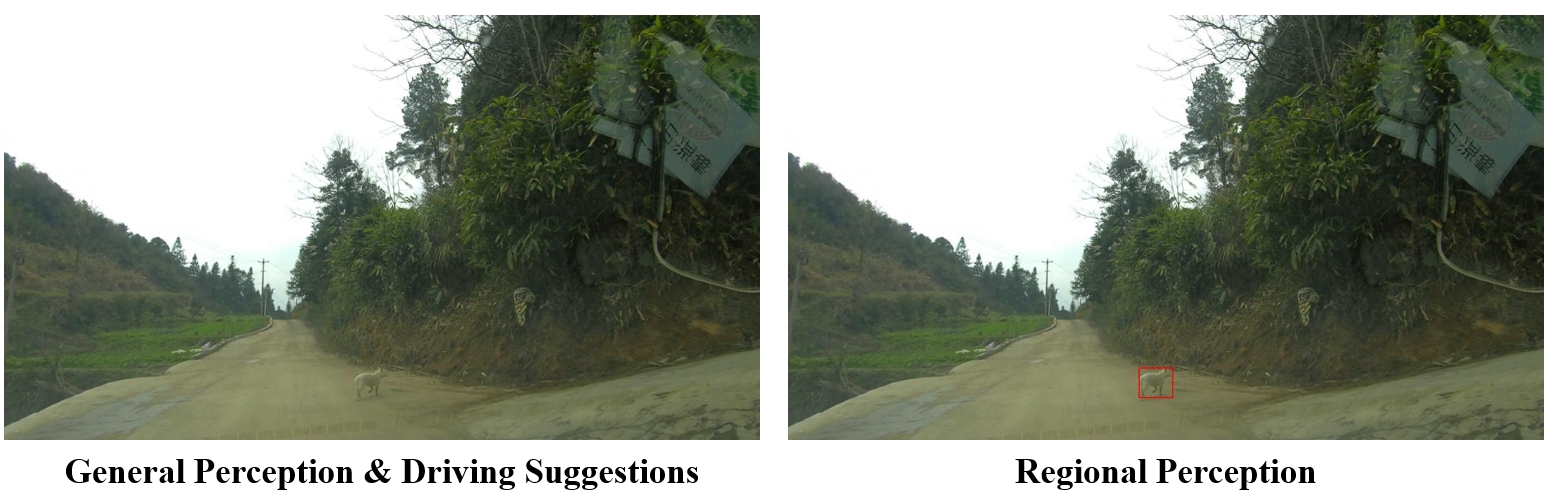
\includegraphics[width=0.8\textwidth]{visual.png} % 插入图片,设置图片宽度为文本宽度的50%
          \caption{区域感知图片示例} % 图片标题
          \label{fig:example} % 图片标签,用于引用
        \end{figure}
\end{enumerate}

\subsubsection{数据评估}
由于最终的评估需要用到商用模型GPT-4o的API,为了控制API调用的成本,我们选择使用CODA-LM的Mini数据集(官方给出的测试集的子集)对LLaVA1.5-7B与LLaVA1.5-13B微调后的模型进行评估。以下是流程概要:

\begin{enumerate}
  \item \textbf{推理与保存结果:}
        按照 CODA-LM 的提交指南,我们分别使用LLaVA1.5-7B与LLaVA1.5-13B微调后的模型对以上转换后的数据执行推理,并按照要求保存结果,推理后的部分结果如图\ref{fig:tuili}所示:
        \begin{figure}[h] % 创建一个图像环境
          \centering % 图片居中
          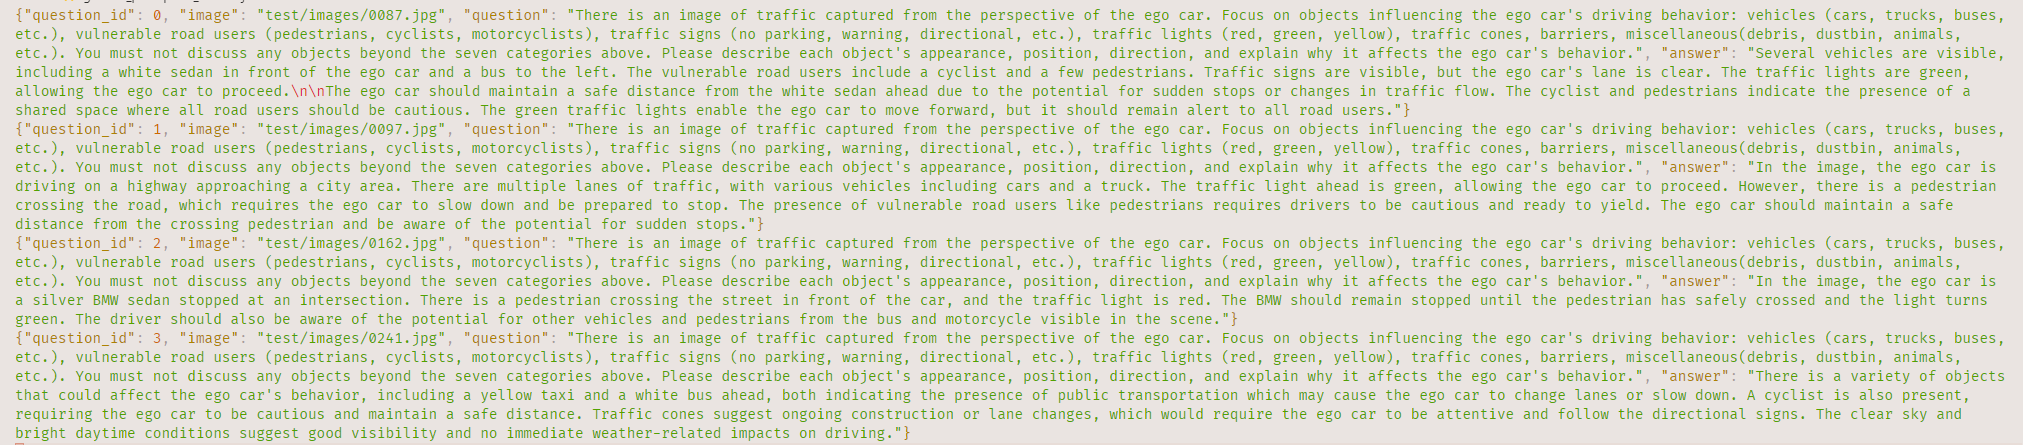
\includegraphics[width=1\textwidth]{tuili.jpg} % 插入图片,设置图片宽度为文本宽度的50%
          \caption{推理部分结果示例} % 图片标题
          \label{fig:tuili} % 图片标签,用于引用
        \end{figure}

  \item \textbf{单独评估每个任务:}
        使用特定的脚本和商用的的GPT-4o模型进行评估,为每个任务生成评估结果:即一般感知、驾驶建议和区域感知三个任务。
    %     \begin{itemize}
    %       \item 一般感知:
    %             \begin{verbatim}
    % python stage1_eval_batch.py --reference_path ./CODA-LM/$ROOT_TO_GT
    %   --prediction_path $ROOT_TO_RESULTS/general_perception_answer.jsonl
    %   --save_path eval/general_perception_answer --model_name gpt-4o-2024-05-13
    %   --api_key $OPENAI_KEY
    % \end{verbatim}
    %       \item 驾驶建议:
    %             \begin{verbatim}
    % python stage2_eval_batch.py --reference_path ./CODA-LM/$ROOT_TO_GT
    %   --prediction_path $ROOT_TO_RESULTS/driving_suggestion_answer.jsonl
    %   --save_path eval/driving_suggestion_answer --model_name gpt-4o-2024-05-13
    %   --api_key $OPENAI_KEY
    % \end{verbatim}
    %       \item 区域感知:
    %             \begin{verbatim}
    % python stage3_eval_batch.py --reference_path ./CODA-LM/$ROOT_TO_GT
    %   --prediction_path $ROOT_TO_RESULTS/region_perception_answer_w_label.jsonl
    %   --save_path eval/region_perception_answer_w_label --model_name gpt-4o-2024-05-13
    %   --api_key $OPENAI_KEY
    % \end{verbatim}
        % \end{itemize}
\end{enumerate}


\subsection{评估结果}
通过以上流程,我们得到了LLaVA1.5-7B与LLaVA1.5-13B微调后的模型在CODA-LM数据集上的评估结果。下表\ref{CODA-LM result}
为比较结果,其中原模型的数据是论文\cite{chen2024automatedevaluationlargevisionlanguage}中给出的,微调后的数据是我们在CODA-LM的Mini集上实验得到的。

对于一般感知的文本得分,微调后的模型(加上 LoRA)在两种规模的版本中都显示出了性能提升。LLaVA1.5-7B 从 19.30 提高到 20.40,LLaVA1.5-13B 从 24.54 提高到 25.00。

区域感知评分分为五个类别:Vehicle(车辆)、VRU(易受伤害路面使用者)、Cone(交通锥)、Barrier(障碍物)、和 Other(其他)。
在 7B 模型中,除了 Vehicle 和 VRU 分数略有下降外,其他三个类别在加上 LoRA 后都有所提升,尤其是 Barrier 和 Other 类别的得分显著增加。在 13B 模型中,加上 LoRA 后 Vehicle 和 VRU 的得分略有下降,但 Barrier 的得分从 30.41 提升至 40.00,显示出较大的增幅。

在驾驶建议方面,加上 LoRA 后的模型在两种规模的版本中都有较大的性能提升,7B 模型从 23.16 提高到 25.20,13B 模型从 27.90 提高到 29.40。

总的来说,LoRA 作为一种低秩适应技术,显著提高了 LLaVA 模型在所有任务的性能,特别是在文本得分和障碍物识别方面。同时,更大规模的模型在没有 LoRA 的情况下就比较小规模的模型表现得更好,这表明更大的模型复杂性有助于提高性能。值得指出的是,虽然在大多数任务中,LoRA 都带来了性能提升,但在特定任务(如 VRU)中,性能有所下降,可能是由于模型在这些特定区域的过拟合或者LoRA适应性的局限。
\begin{table}[htbp]
  \centering
  \caption{Comparison of LLaVA model before and after fine-tuning on CODA-LM dataset}
  \label{CODA-LM result}
  \small % 调整表格字体大小
  % \renewcommand{\arraystretch}{1.2} % 调整行距
  \begin{tabular}{lcccccccccc}
    \toprule
    \textbf{Method}   & \textbf{General↑}   & \multicolumn{5}{c}{\textbf{Regional Perception↑}} & \textbf{Suggestion↑}                                                                           \\
    \cmidrule(r){3-7}
                      & \textbf{Text-Score} & \textbf{Vehicle}                                  & \textbf{VRU}         & \textbf{Cone} & \textbf{Barrier} & \textbf{Other} & \textbf{Text-Score} \\
    \midrule
    LLaVA1.5-7B       & 19.30               & 46.67                                             & 38.47                & 50.83         & 30.93            & 33.82          & 23.16               \\
    LLaVA1.5-7B+LoRA  & \textbf{20.40}      & 46.03                                             & 36.00                & 45.56         & \textbf{33.57}   & \textbf{40.00} & \textbf{25.20}      \\
    \midrule
    LLaVA1.5-13B      & 24.54               & 53.62                                             & 36.79                & 41.27         & 30.41            & 33.82          & 27.90               \\
    LLaVA1.5-13B+LoRA & \textbf{25.00}      & 53.45                                             & 30.00                & 41.11         & \textbf{40.00}   & \textbf{34.29} & \textbf{29.40}      \\
    \bottomrule
  \end{tabular}
\end{table}



\section{实验结论}

\appendix
\newpage
\section*{参考文献}
\addcontentsline{toc}{section}{参考文献}
\printbibliography[heading=none]
% \noindent
% [1] 乐东明,王文浚,王颖,等. 2020—2022年咸宁市臭氧污染气象特征及成因分析[J].黑龙江环境通报, 2024, 37(05):30-32.

% \noindent
% [2] 李高荣,吴密霞. 多元统计分析[M]. 北京:科学出版社, 2021

% \noindent
% [3] John A. Rice. Mathematical Statistics and Data Analysis[M]. Boston: Cengage Learning, 2006

% \noindent
% [4] 何书元. 应用时间序列分析[M]. 北京:北京大学出版社, 2003

\newpage
\section*{附录:实验日志与心得}
\addcontentsline{toc}{section}{附录:实验日志与心得}

\end{document}